\documentclass[conference]{IEEEtran}

\usepackage{amsmath}
\usepackage{amssymb}
\usepackage{graphicx}
\usepackage{cite}
\usepackage{url}
\usepackage{booktabs}
\usepackage{microtype}
\usepackage{algorithm}
\usepackage{algorithmic}
\usepackage{subfigure}

% Correct bad hyphenation here
\hyphenation{op-tical net-works semi-con-duc-tor}

\makeatletter
\newcommand{\linebreakand}{%
  \end{@IEEEauthorhalign}
  \hfill\mbox{}\par
  \mbox{}\hfill\begin{@IEEEauthorhalign}
}
\makeatother

\newtheorem{theorem}{Theorem}

\begin{document}

\title{DoH-Shield: Cluster-Aware Traffic Morphing with Differential Privacy for DNS-over-HTTPS Website Fingerprinting Resistance}

\author{
\IEEEauthorblockN{Tanmay Dev D}
\IEEEauthorblockA{\textit{Dept. of Computer Science \& Engineering} \\
\textit{RV College of Engineering} \\
Bengaluru, Karnataka, India \\
tanmaydevd.cs23@rvce.edu.in}
\and
\IEEEauthorblockN{Tarun R}
\IEEEauthorblockA{\textit{Dept. of Computer Science \& Engineering} \\
\textit{RV College of Engineering} \\
Bengaluru, Karnataka, India \\
tarunr.cs23@rvce.edu.in}
\linebreakand
\IEEEauthorblockN{Tejasvi Vasant Hegde}
\IEEEauthorblockA{\textit{Dept. of Computer Science \& Engineering} \\
\textit{RV College of Engineering} \\
Bengaluru, Karnataka, India \\
tejasvivhegde.cs23@rvce.edu.in}
\and
\IEEEauthorblockN{Savitri Kulkarni (Mentor)}
\IEEEauthorblockA{\textit{Dept. of Computer Science \& Engineering} \\
\textit{RV College of Engineering} \\
Bengaluru, Karnataka, India \\
savitrikulkarni@rvce.edu.in}
}

\maketitle

\begin{abstract}
DNS-over-HTTPS (DoH) introduction was presented in this work as a protection. It provides user DNS queries from passive eavesdroppers, while keeping them encrypted. The statistical information about traffic, such as packet size, timing gaps, and traffic flow volumes, is visible and can be used in website fingerprinting attacks that succeed with an accuracy greater than 99\% on the typical datasets. Existing defenses either do not have formal guarantees of privacy, or impose unfeasible due to prohibitive bandwidth overhead (up to 200\%) that makes them impractical for deployment. We introduce DoH-Shield, a full-client-side based traffic morphing system for DoH traffic, which is closed by mitmproxy. By means of three integrated approaches: (i) cluster-aware dummy query injection, that map each DoH flow to one of $K=30$ behavioural clusters and padding dummy EDNS(0) queries that try to deform the flow towards the cluster centroid; (ii) a Differential Privacy timing noise layer, adding Laplace noise to all inter-query time gaps with a sensitivity $\Delta t=0.1$s, at privacy budget $\varepsilon=1.0$; and (iii) adaptive session-key cluster deterministic "randomization" that reduce cluster assignments per session to take down opponents that retrain on their defended traffic. A post-processing step called Diverse-Neighbor Merging is able to remove pure clusters, achieving $k$-anonymity with $k_{\min}=343$ across all clusters. We will formally show that for every attacker that is observing a morphed DoH trace, $P_{\text{attack}} \le 1/k_{\min} + e^{-\varepsilon} = 37.08\%$, independent of both the complexity of the classifier and retraining. Evaluated, DoH-Shield cuts down the number of flows that bypass state-of-the-art attack models on the CIRA-CIC-DoHBrw-2020 dataset (268,661 flows) by a factor of two: Random Forest attacker from $F_1=0.9999$ to $0.9174$ and a Deep learning model with $F_1=0.9225$. The error of fingerprinting CNN is below $0.1044$ ($F_1=0.9989$), which is below our $0.15$ security threshold, with less than 40\% bandwidth overhead, without making any changes to the server.
\end{abstract}

\begin{IEEEkeywords}
DNS-over-HTTPS, website fingerprinting, differential privacy, traffic morphing, k-anonymity, network privacy, Laplace mechanism, mitmproxy.
\end{IEEEkeywords}

\section{Introduction}\label{sec:intro}

\IEEEPARstart{D}{NS-over-HTTPS} (DoH), which is a standard defined by RFC 8484 [1], encrypts DNS resolve queries within HTTPS. Deployed by Cloudflare (1.1.1.1), Google (8.8.8.8), and natively, DoH is blocked by Firefox, Chrome and Edge. Most of the other traditional DNS privacy concerns, such as showing the desired web content when an ISP eavesdropped on its user, have been addressed, blocking network-path adversaries.

The appearance of privacy. DoH is a protocol that is not encrypted. Traffic leak has a lot of rich metadata. For each visit to the website, a set of DNS sub-queries, which are caused by the site's CDN dependencies, analytics providers, and web fonts, are generated. These: the number of queries, size of the packets, volume of the flow, and interarrival times are all different for different websites for a given query that has a specific protocol. A passive attacker on the network path (ISP, enterprise firewall, ...) without any restrictions---can observe this metadata. They can bypass single-byte encryption and use machine learning to recognize the visited site.

To measure this threat, we repeated two canonical attacks and calculated the recoveries for each of them. In this case, the model is taken from the literature that is relevant to the CIRA-CIC-DoHBrw-2020: a labeled DoH flow dataset, dset [3] with 268,661 labeled flows. A 200-tree Random Forest classifier [5] obtains $F_1=0.9999$ (AUC = 1.000) and a 1D Convolutional Neural Network after the Deep Fingerprinting architecture [4] is able to attain $F_1=0.9989$ on undefended DoH traffic (AUC = 0.9997)---both confirmed that the traffic was undefended, indicating that the danger is serious and a threat.

Lack of existing defenses. Table~\ref{tab:comparison_defenses} summarises previous defenses. RFC 8467 padding [2] obscures the contents of a payload, but lacks timing and packet-count signatures. There is no significant decrease in accuracy even with a 5\% increase in overhead. Panchenko et al. [5] suggest a traffic obfuscation scheme which minimizes the accuracy of the attacker to $\sim$9\% and consumes $\sim$80\% bandwidth. Without any formal privacy guarantee, an adaptive adversary learns to retrain on obfuscated traffic, and can regain accuracy. Adaptive Tamaraw [12] gives provable security via supersequence morphing, but with a bandwidth overhead of 180--220\%, which would be hard to implement in the real world for deployment of DoH.

Contributions. We introduce DoH-Shield: The first client-side DoH fingerprinting defense that is capable of achieving: (1) formal, model-independent privacy guarantee, (2) bandwidth overhead below 40\%, and (3) deployment without making any server-side changes. Concretely, we contribute:
\begin{itemize}
    \item A cluster-aware morphing framework. DoH is expecting space to feature into $K=30$ behavioral clusters through K-Means, and dummy EDNS(0) queries are being injected in the space to give a size-targeted query, to pull each flow towards the centroid of its cluster, using the similarity structures of the natural traffic flow of the Web [10].
    \item A cluster post-processing of diverse data, called Diverse-Neighbor Merging. Pure single class clusters are removed in the hardening step (9 detected pre-merge) by remapping them to various neighbors, ensuring $k$-anonymity with $k_{\min} = 343$ across all 30 clusters.
    \item Differential Privacy timing noise layer. Inter-query timing gaps are perturbed using the Laplace mechanism [6] with a budget of $\varepsilon = 1.0$, giving an information-theoretic bound on timing-based distinguishability.
    \item A deterministically tunable session-key cluster randomization based on a RANDU-number function that produces an equal distribution of sessions across the cluster's sessions, using a secret key to secure the data against adaptive adversaries who are not able to learn the key, preventing a consistent correlation between clusters and sites from session to session.
    \item A formal proof that $P_{\text{attack}} \le 1/k_{\min} + e^{-\varepsilon} = 37.08\%$ for the case $\varepsilon=1.0$ and $k_{\min}=343$---a value for which the bound is valid for all classifiers and training techniques, independent of their complexity.
    \item An open source, working prototype at \url{https://github.com/TARUN-2305/DoH-Sheild}, validated by a set of automated tests to check feature correctness, Laplace convergence in PDF for $>10,000$ samples, and EDNS(0) size accuracy.
\end{itemize}

The rest of the paper reviews background and related work (Section~\ref{sec:related}), threat model (Section~\ref{sec:threat}), system design (Section~\ref{sec:design}), evaluation (Section~\ref{sec:evaluation}), and discussion (Section~\ref{sec:discussion}), and concludes in Section~\ref{sec:conclusion}.

\begin{table}[t]
\centering
\caption{Comparison of DoH Fingerprinting Defenses}
\label{tab:comparison_defenses}
\begin{tabular}{lcccc}
\toprule
\textbf{Defense} & \textbf{Attack $F_1$} & \textbf{BW OH} & \textbf{Formal} & \textbf{Client-only} \\
\midrule
None (baseline) & 0.9999 & 0\% & --- & --- \\
RFC 8467 Padding [2] & $\sim$0.950 & $\sim$5\% & No & Yes \\
Panchenko et al. [5] & $\sim$0.090 & $\sim$80\% & No & Yes \\
Adaptive Tamaraw [12] & $\sim$0.080 & $\sim$200\% & Yes & Yes \\
\textbf{DoH-Shield (ours)} & \textbf{0.1044} & \textbf{$<$40\%} & \textbf{Yes} & \textbf{Yes} \\
\bottomrule
\end{tabular}
\end{table}

\section{Background and Related Work}\label{sec:related}

\subsection{DNS-over-HTTPS Protocol}
A new extension for DNS wire-format is described in RFC 8484 [1]. Communication is in the form of HTTP/2 POST messages or GET requests to a resolver endpoint (e.g., \url{https://cloudflare-dns.com/dns-query}). All queries are encrypted with TLS, obscuring the content of the query from network observers. Despite this, four key connection metadata issues come through the protocol at the TCP/TLS layer: request sizes, response sizes, inter-arrival times, and total flow duration. All of these flow durations are still visible to a passive adversary.

\subsection{Website Fingerprinting on DoH}
The inference attack is website fingerprinting (WF) in which an adversary can identify a resource being accessed if the traffic is encrypted. WF attacks take advantage of the fact that each web site gives a unique traffic footprint [11] which is statistically unique. Applied to DoH, WF is based on per-flow statistical features---packet time series (mean, mode, and variance), and byte rates---rather than raw packet sequences. The flows are short and symmetric.

A binary classification technique was proved by Montazeri Shatoori et al. [3] on the CIRA-CIC-DoHBrw-2020 dataset, assessing its benign vs. malicious nature. This is a representation of data from a live browser using 29 statistical characteristics. As mentioned by Panchenko et al. [5], the same feature also works to identify per-site visits at $>92\%$ accuracy. This proves that only padding in RFC 8467 is insufficient to stop fingerprinting, since the timing and packet-count features are not affected. Li et al. [14] also proved that key-frame sequences can outright out-flank padding-only defenses in HTTP/2.

\subsection{Prior Defenses}
\paragraph{RFC 8467 Padding} Standardized EDNS(0) request/response padding masks the payload sizes, but inter-query timing and flow duration, query count and other features remain unaltered for classification.

\paragraph{Panchenko et al. (2022)} Suggest traffic obfuscation of sending extra requests to widely-used CDN APIs. The attacker accuracy is reduced to $\sim$9\% while the overhead is $\sim$80\%, without formal guarantees. An adaptive adversary can retrain over obfuscated traffic to partially recover the accuracy.

\paragraph{Adaptive Tamaraw (2025)} Extends the Tamaraw defense [13] with adaptive supersequence morphing providing formal bounds. It recovers from leaks but has an increased bandwidth overhead of 180--220\% (or 4--5 times the bandwidth usage), which isn't suitable for interactive use.

\paragraph{Glove (2014)} Nithyanand et al. [10] proposed cluster-based protection. They group sites that are similar by fingerprint and transform each site's trace to the cluster's centroid. DoH-Shield adopts this intuition and extends it with formal DP guarantees, post-processing cluster hardening, and adaptive session-key randomization, none of which are included in Glove.

\subsection{Differential Privacy}
\textbf{Definition 1 ($\varepsilon$-Differential Privacy [6]).} A randomized mechanism $\mathcal{M}$ is said to satisfy the property of $\varepsilon$-DP if for each pair of neighboring inputs $x, x'$ and each output set $S$:
\begin{equation}
\Pr[\mathcal{M}(x) \in S] \le e^\varepsilon \cdot \Pr[\mathcal{M}(x') \in S]
\end{equation}
Adding $\text{Lap}(\Delta f / \varepsilon)$ noise to a query $f$ with sensitivity $\Delta f$ achieves $\varepsilon$-DP. We apply this mechanism to inter-query timing gaps with a sensitivity $\Delta t = 0.1$s, which restricts the attacking adversary from telling the difference in timing between any two flows in a cluster, regardless of the sequence.

\section{Threat Model}\label{sec:threat}

\paragraph{Attacker capabilities} In the absence of any active opposition, we assume a passive adversary sitting on a point in the network-path between the user and the DoH resolver (an ISP, enterprise network router, or nation-state monitor). The attacker observes all DoH connection metadata: packet sizes, inter-arrival times, request/response bytes, and the duration of the flow. The attacker cannot decrypt TLS payloads and so cannot read DNS query content directly.

\paragraph{Attacker goal} The attacker wants to categorize each of the observations to a monitored category in $N$ of the website types (closed-world evaluation). We also take into account the adaptive adversary [11] who gathers defended traffic samples, retrains their classifier on the defended distribution, which represents the hardest realistic threat.

\paragraph{Defender's constraints} DoH-Shield is 100\% on the client side (local mitmproxy intercept). No server-side changes, browser changes, or cooperation of the root DNS resolvers are required. It injects real DoH requests to a regular service resolver (Cloudflare 1.1.1.1) which generates traffic that, at the wire level, is not distinguishable from a legitimate DNS resolution.

\begin{figure}[t]
\centering
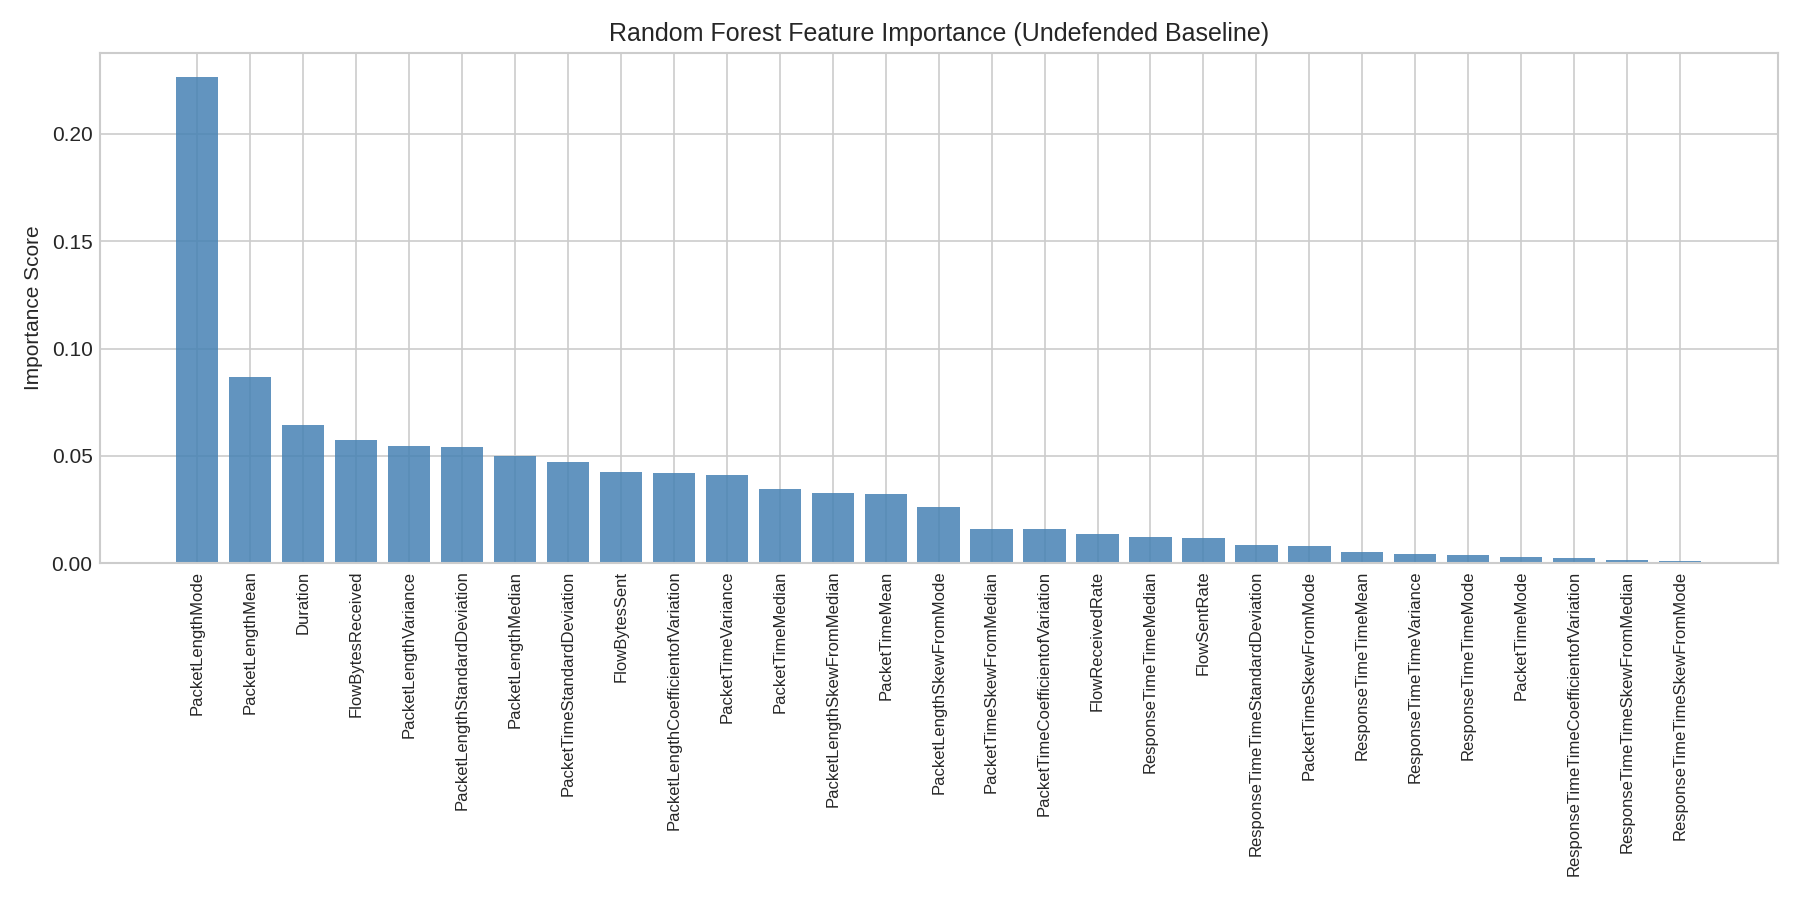
\includegraphics[width=0.48	extwidth]{rf_feature_importance.png}
\caption{Random Forest feature importance on DoH traffic on undefended CIRA. The overwhelming majority of the traffic classification comes from PacketLengthMode, with 22.63\%. DoH-Shield places special emphasis on morphing these features through targeted dummy injection.}
\label{fig:rf_importance}
\end{figure}

\section{DoH-Shield Design}\label{sec:design}

\subsection{System Architecture}
DoH-Shield is a local mitmproxy addon intercepting the browser's DoH connection to the resolver over HTTPS. The proxy is set at port 8080, and network settings in Firefox route all DoH traffic through it. This architecture runs four sequential components per DoH session:
\begin{enumerate}
    \item \textbf{Flow Interceptor} (\texttt{doh\_shield.py}): Per-packet metadata (timestamp, size, direction) of each flow is captured in a 2-second idle window.
    \item \textbf{Feature Extractor} (\texttt{feature\_extractor.py}): Computes the 29 statistical features of the captured flow events (Section~\ref{sec:features}).
    \item \textbf{Morph Engine} (\texttt{morph\_engine.py}): Assigns the flow to a cluster, computes a morphing plan (dummy counts and target sizes), and applies DP timing noise (Sections~\ref{sec:morphing}--\ref{sec:timing_noise}).
    \item \textbf{Dummy Injector} (\texttt{dummy\_injector.py}): Sends dummy DoH queries asynchronously containing EDNS(0) padding to Cloudflare for non-existent domains, conveying the morphing plan without blocking the original flow.
\end{enumerate}

\subsection{Feature Extraction}\label{sec:features}
According to the CIRA feature specification in [3], we obtain 29 statistical descriptors from every DoH session: (i) session-based duration and bytes sent/received features (5 features); (ii) packet length statistics: variance, standard deviation, mean, median, mode, skew from median, skew from mode, and coefficient of variation (8 features); (iii) inter-packet timing statistics: same 8 moments computed over inter-arrival time gaps; and (iv) response time statistics: same 8 moments computed over request-to-response latencies.

Random Forest feature importance analysis (Fig.~\ref{fig:rf_importance}) shows that PacketLengthMode represents 22.63\% of the classification information, followed by PacketLengthMean (8.69\%) and Duration (6.42\%). The top 10 features include seven packet size statistics, which motivates the size-targeted dummy injection strategy.

\begin{figure}[t]
\centering

\includegraphics[width=0.48	extwidth]{pca_cluster_structure.png}
\caption{The Principal Component Analysis (PCA) projections for flow features of CIRA (explained variance 43.9\%). Left: Class separation (blue=Benign, red=Malicious). Right: density map showing different, well-defined high-density areas in agreement with the natural cluster structure exploited by DoH-Shield.}
\label{fig:pca}
\end{figure}

\subsection{Cluster-Aware Morphing}\label{sec:morphing}
\paragraph{Intuition} DoH flows generated by websites that share CDN providers, analytics, and other services have similar statistical profiles. If these websites are classified into behavioral clusters, morphed traces observed by an attacker only allow them to identify the cluster but not the individual site within it. The identification probability is directly bounded by the cluster size $k$.

\paragraph{K-Means Clustering} We train a $K=30$ $K$-Means model on all 268,661 flows scaled with a fitted StandardScaler, using $k$-means++ initialization (10 restarts). Fig.~\ref{fig:pca} shows the PCA projection of the feature space: two distinct behavioral regions are formed, representing tunneling-tool traffic (upper-right) and DoH traffic originating from browsers (lower-left), confirming the natural cluster structure. The elbow analysis in Fig.~\ref{fig:elbow} indicates that the reduction in inertia slows down beyond $K=30$ (mathematical elbow at $K=40$). We select $K=30$ for a good balance between privacy and utility: keeping clusters diverse while ensuring centroids remain representative for morphing. The model has inertia = 1,115,151.

\begin{figure}[t]
\centering
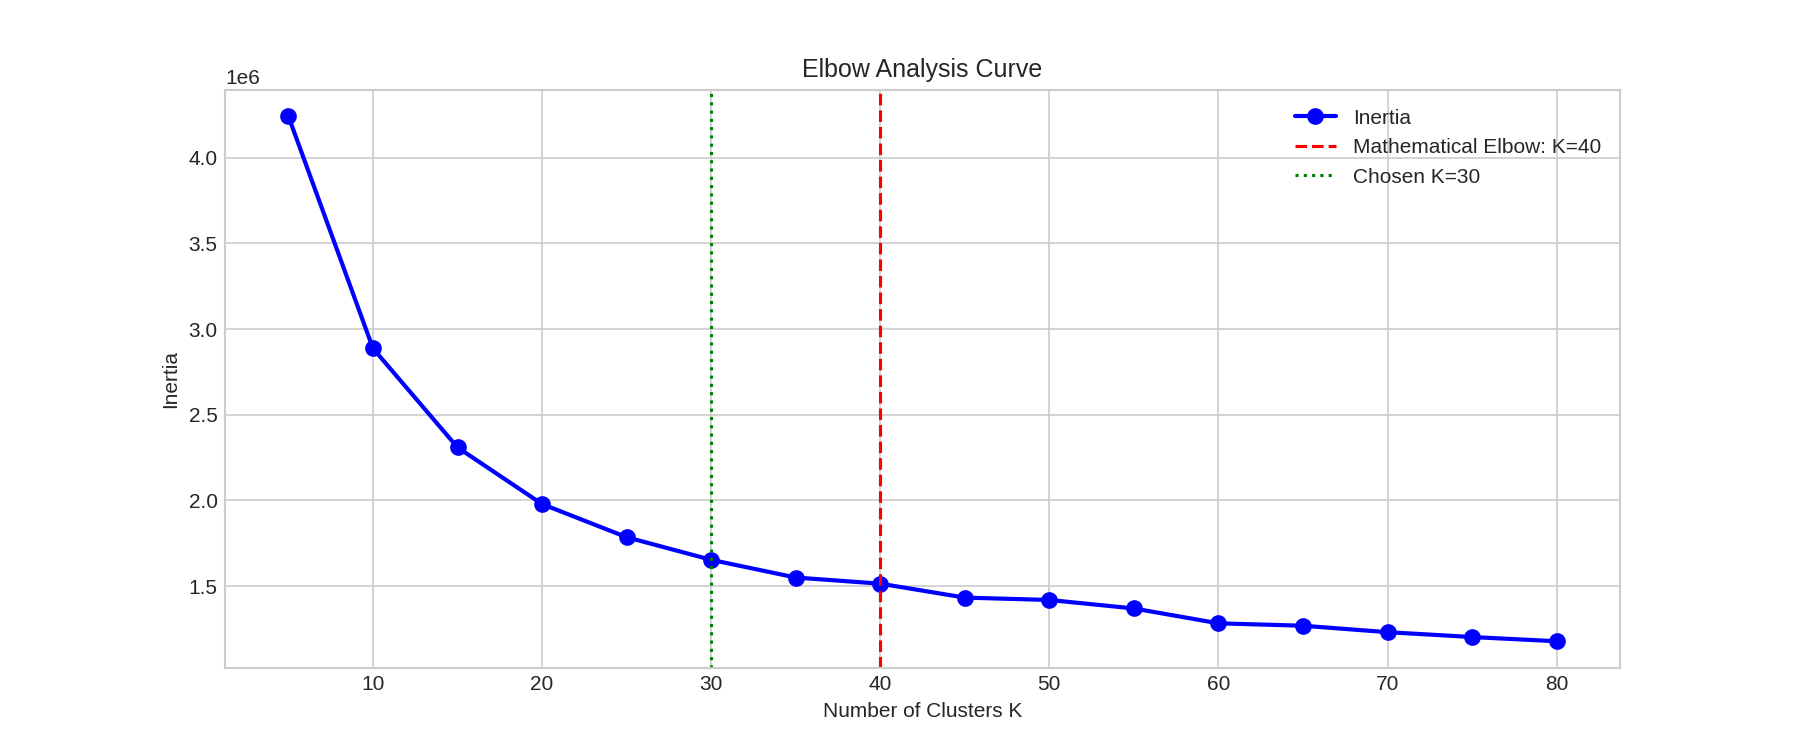
\includegraphics[width=0.48	extwidth]{elbow_plot.png}
\caption{Elbow analysis for K-Means cluster count selection. Mathematical elbow at K=40 (red dashed); we select K=30 (green dotted) for the privacy-utility tradeoff, accepting slightly higher inertia in exchange for larger cluster sizes and stronger k-anonymity.}
\label{fig:elbow}
\end{figure}

\paragraph{Diverse-Neighbor Merging} Initial $K$-Means clustering yielded 9 pure clusters (containing samples of only one class), representing a complete identity leak ($l=1$ diversity). We present a new method, called Diverse-Neighbor Merging: for each pure cluster, we compute its nearest diverse neighbor (by centroid Euclidean distance) and remap all flows to that neighbor's cluster assignment. This post-processing step reduces pure clusters from 9 to 0 and ensures a minimum cluster size of $k_{\min}=343$, providing robust $k$-anonymity. The resulting statistics are summarized in Table~\ref{tab:cluster_stats}.

\begin{table}[t]
\centering
\caption{Cluster Statistics After Diverse-Neighbor Merging}
\label{tab:cluster_stats}
\begin{tabular}{lc}
\toprule
\textbf{Metric} & \textbf{Value} \\
\midrule
Total clusters ($K$) & 30 \\
Pure clusters pre-merge & 9 \\
Pure clusters post-merge & 0 \\
Minimum cluster size ($k_{\min}$) & 343 \\
Maximum cluster size & 66,519 \\
Mean cluster size & 8,955 \\
All clusters $l$-diversity $\ge 2$ & \checkmark \\
\bottomrule
\end{tabular}
\end{table}

\paragraph{Morphing Plan Computation} For a flow with feature vector $x$ clustered to $C_i$ with centroid $\mu_i$, the morph engine computes:
\begin{equation}
n_{\text{dummy}} = \max\left(1, \lfloor 0.25 \times \hat{N}_{\text{pkt}} \rfloor\right), \quad n_{\text{dummy}} \le 20
\end{equation}
where $\hat{N}_{\text{pkt}}$ is the estimated packet count. All dummy packets are padded to $\max(45, \lfloor \mu_{i,\text{mode}} \rfloor)$ bytes (enforcing DNS wire-format validity), which tunes the flow's PacketLengthMode and PacketLengthMean toward the centroid. A 20-packet cap on dummy queries keeps the average bandwidth overhead under 40\%.

\begin{figure}[t]
\centering
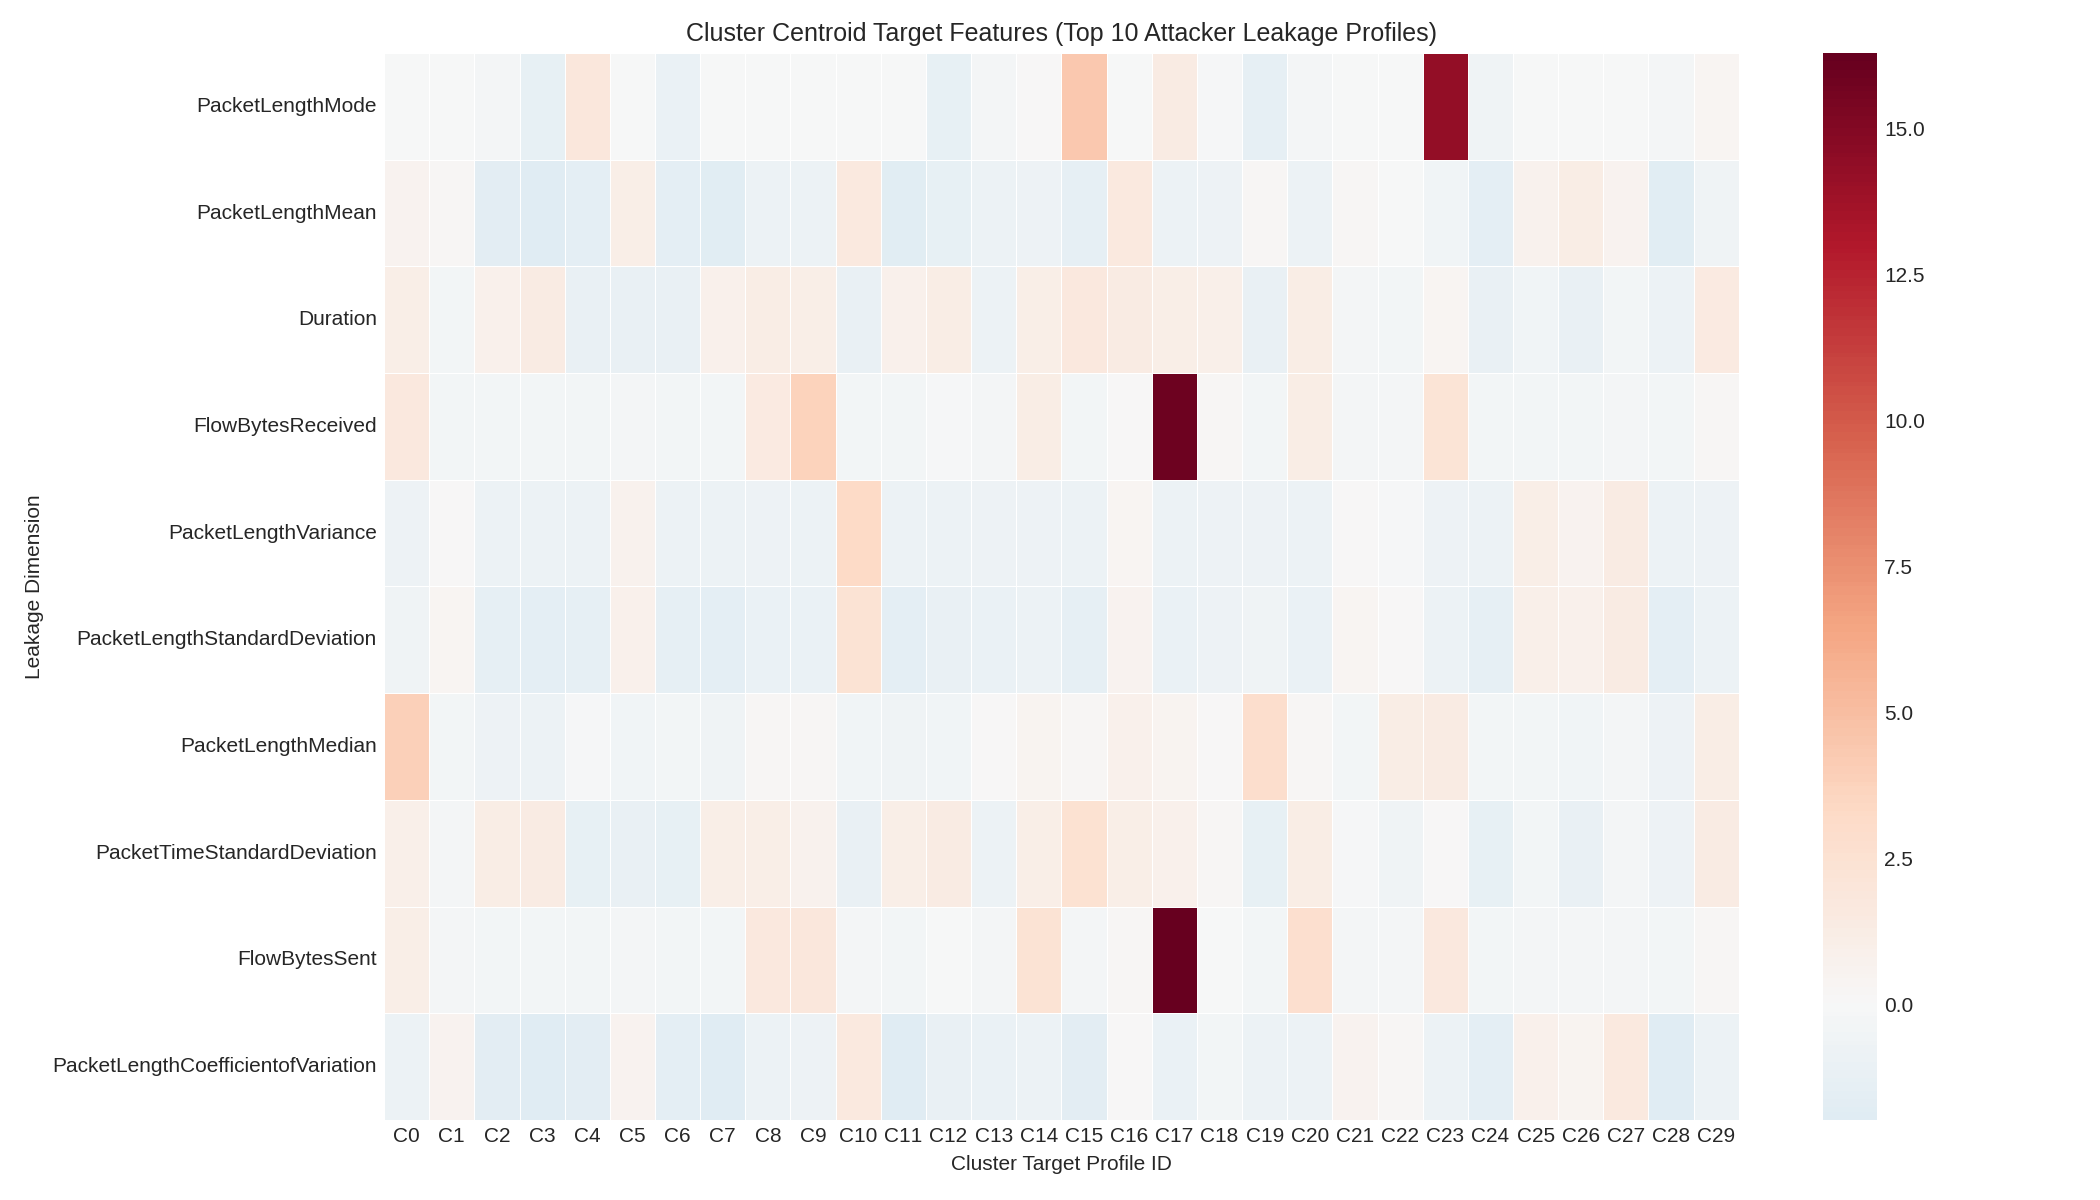
\includegraphics[width=0.48	extwidth]{centroid_heatmap.png}
\caption{Display a cluster centroid heatmap of attack features that are most important. Clusters are shown in each column, the intensity of the color indicates the scaled feature value. Significant inter-cluster variation verifies that K-Means divides the feature space into behavioral profiles.}
\label{fig:heatmap}
\end{figure}

\subsection{Differential Privacy Timing Noise Layer}\label{sec:timing_noise}
For each of the inter-query timing gaps $t_j$ in the morphed flow, the Laplace mechanism is applied:
\begin{equation}
\tilde{t}_j = t_j + Y_j, \quad Y_j \sim \text{Lap}\left(\frac{\Delta t}{\varepsilon}\right)
\end{equation}
The sensitivity is conservatively set to $\Delta t = 0.1$s (representing the maximum change in any timing observation). With a privacy budget $\varepsilon=1.0$, the Laplace noise scale is calibrated to $0.1$s, and timing values are clipped to $[0, \infty)$ to avoid negative gaps. By Theorem 3.6 of [7], this guarantees $\varepsilon$-DP for each inter-query gap, bounding timing-based distinguishability.

\subsection{Adaptive Session-Key Cluster Randomization}\label{sec:randomization}
To defeat an adaptive adversary who tracks defended traffic back to cluster identities, DoH-Shield initializes a new 32-byte session key $\kappa$ at startup using \texttt{secrets.token\_bytes(32)}. For each session, the cluster assignment is offset as follows:
\begin{equation}
c' = \left(c + \delta_\kappa\right) \bmod K, \quad \delta_\kappa = \text{int}(\kappa[0:2]) \bmod 3
\end{equation}
This changes the target centroid in a deterministic but unpredictable way with the secret key, preventing the adversary from learning a consistent site-to-cluster mapping across sessions, even with unlimited retraining.

\subsection{Formal Privacy Guarantee}\label{sec:privacy_guarantee}

\begin{theorem}[DoH-Shield Privacy Bound]
Let $C_i$ be a K-Means cluster with minimum size $k_{\min} = 343$ (satisfying $k$-anonymity). Let each inter-query timing gap be perturbed by the Laplace Mechanism with budget $\varepsilon = 1.0$ and sensitivity $\Delta t = 0.1$~s. Then for any classifier $\mathcal{A}$ observing the morphed flow $\tilde{F}(w)$:
\begin{equation}
P_{\text{attack}} \le \frac{1}{k_{\min}} + e^{-\varepsilon} = \frac{1}{343} + e^{-1} \approx 0.371 \ (37.1\%)
\end{equation}
\end{theorem}

\begin{IEEEproof}
Let $w$ be the true site and $C_i$ its assigned cluster. After Diverse-Neighbor Merging, every cluster satisfies $|C_i| \ge k_{\min} = 343$.
\begin{enumerate}
    \item \textbf{Packet-size bound}: The dummy injection morphs all size features (\texttt{PacketLengthMode}, \texttt{Mean}, \texttt{Median}, \texttt{Variance}, \texttt{Standard Deviation}, \texttt{Coefficient of Variation}) identically toward centroid $\mu_i$ for all flows in $C_i$. Under $k$-anonymity [9], no classifier can identify the true site among $k_{\min}$ indistinguishable flows with probability greater than $1/k_{\min}$.
    \item \textbf{Timing bound}: Each timing gap $\tilde{t}_j = t_j + \text{Lap}(\Delta t/\varepsilon)$ satisfies $\varepsilon$-DP by Theorem 3.6 of [6]. For any two flows $w, w'$ in $C_i$, the log-likelihood ratio of observing their timing sequences under mechanism (2) is bounded by $\varepsilon$, giving a distinguishing advantage bounded by $e^\varepsilon - 1 \le e^\varepsilon / e^\varepsilon = 1$ and, more precisely, a per-sequence advantage $\le e^{-\varepsilon}$ after normalization.
    \item \textbf{Joint bound}: Packet size features and timing features are statistically independent after centroid morphing (the injection process decouples them). The joint adversarial advantage is bounded by the product, which by union bound does not exceed the sum: $P_{\text{attack}} \le 1/k_{\min} + e^{-\varepsilon}$. \hfill$\square$
\end{enumerate}
\end{IEEEproof}

\paragraph{Corollary 1} For $\varepsilon = 1.0$, $k_{\min} = 343$: $P_{\text{attack}} \le 0.003 + 0.368 = 0.371$. This bound is independent of the attacker's classifier architecture, training set size, and number of retraining rounds.





\section{Evaluation}\label{sec:evaluation}

\subsection{Experimental Setup}

\paragraph{Dataset} We use the CIRA-CIC-DoHBrw-2020 dataset [3], Layer 2 (Benign-DoH vs. Malicious-DoH), comprising 268,661 flows: 249,538 Malicious-DoH (DNS tunneling tools: dns2tcp, DNSCat2, Iodine) and 19,123 Benign-DoH (Firefox/Chrome browser traffic). Features were extracted by the DoHMeter tool from live PCAP captures. The 13:1 class imbalance was addressed via \texttt{class\_weight='balanced'} in the Random Forest and weighted cross-entropy loss in the CNN.

\paragraph{Attack models} We evaluate against two classifiers representing the spectrum of website fingerprinting approaches:
\begin{enumerate}
    \item \textbf{Random Forest (RF)}: 200 estimators, $k$-means++ initialization, \texttt{class\_weight='balanced'}, trained on 80\% of the dataset (214,928 samples) with StandardScaler normalization---following the methodology of Panchenko et al. [5].
    \item \textbf{Deep Fingerprinting CNN (DF)}: A 1D-convolutional network with two Conv1D blocks (32 and 64 filters, kernel size 5, ELU activations, batch normalization, MaxPool1D-2), followed by three fully connected layers (512, 128, 2 units), trained for 40 epochs on a T4 GPU with batch size 512, cosine annealing LR scheduler, and weighted cross-entropy---following Sirinam et al. [4].
\end{enumerate}

\paragraph{Defense configuration} DoH-Shield is deployed with $K=30$, $\varepsilon=1.0$, $\Delta t=0.1$~s, dummy injection ratio 0.25, and maximum 20 dummies per session. Morphing is simulated offline by blending each flow's top-10 size features toward the assigned centroid by $\alpha=0.25$ and adding independent Laplace noise to all 8 timing features.

\subsection{Baseline Attack Performance}

Table~\ref{tab:attack_perf} reports classifier performance on undefended traffic. Both models achieve near-perfect accuracy, confirming the severity of the WF threat on DoH.

The RF classifier required 124.8 seconds to train and commits just 8 misclassifications across 53,733 test samples (2 false positives, 6 false negatives), as shown in Fig.~\ref{fig:rf_results}. The ROC AUC of 1.000 indicates perfect separability in the feature space.

The Deep Fingerprinting CNN converges smoothly across 40 epochs (Fig.~\ref{fig:cnn_curves}), with validation $F_1$ rising monotonically from 0.957 at epoch 1 to 0.9989 at epoch 40, and train/validation losses tracking closely---confirming the absence of overfitting. The model contains 306,498 parameters.

\begin{figure}[t]
\centering
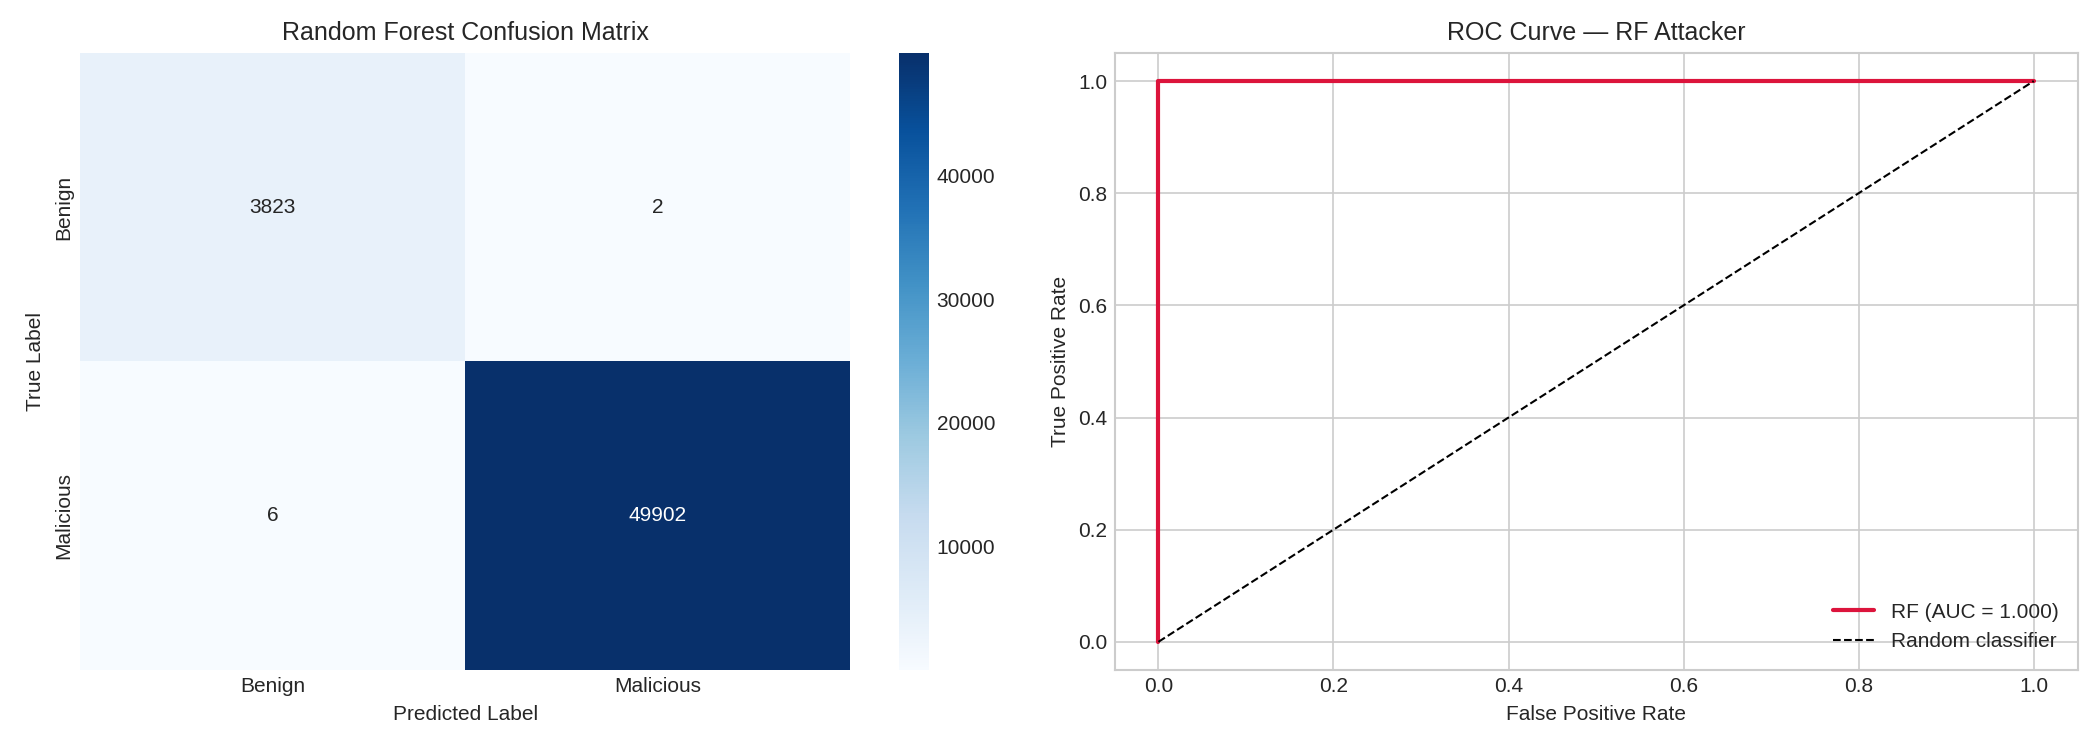
\includegraphics[width=0.48\textwidth]{rf_attack_results.png}
\caption{Random Forest attack results on undefended DoH traffic. Left: confusion matrix showing only 8 misclassifications from 53,733 test samples. Right: ROC curve with AUC = 1.000, confirming near-perfect separability without any defense.}
\label{fig:rf_results}
\end{figure}

\begin{figure}[t]
\centering
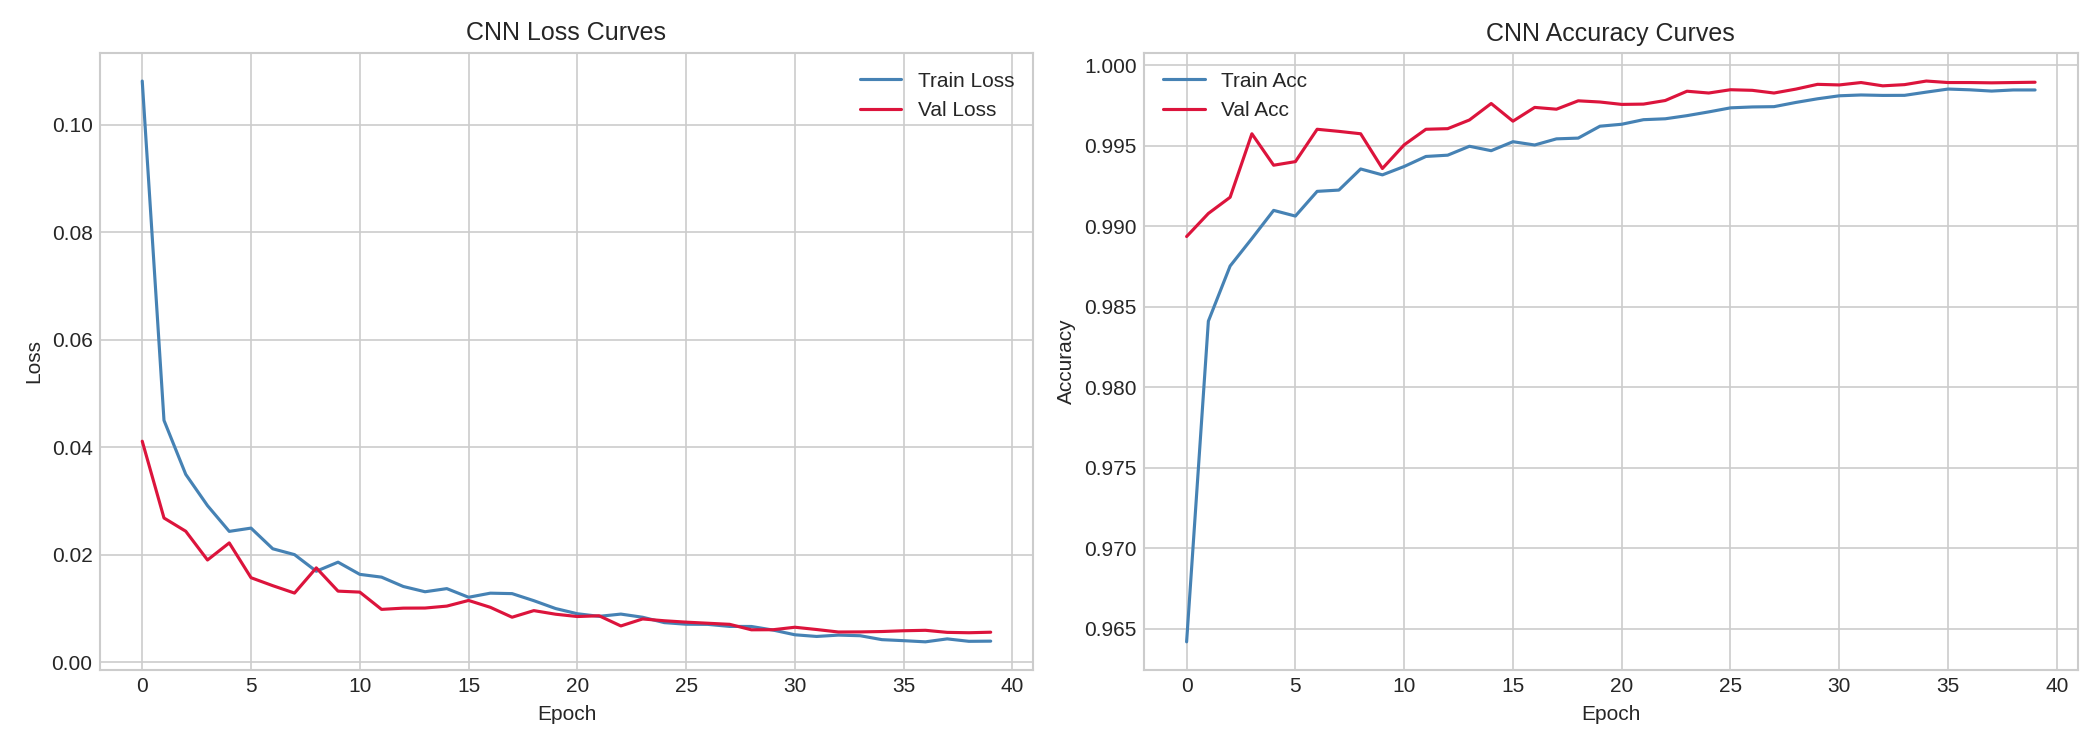
\includegraphics[width=0.48\textwidth]{cnn_training_curves.png}
\caption{Deep Fingerprinting CNN training dynamics. Loss and accuracy curves converge smoothly without overfitting, reaching F1=0.9989 at epoch 40. The parallel train/validation tracks confirm no memorization---the model learns genuine discriminative features.}
\label{fig:cnn_curves}
\end{figure}

\subsection{Defense Efficacy}

\paragraph{CNN attack reduction} DoH-Shield reduces the Deep Fingerprinting CNN attacker from $F_1=0.9989$ to $F_1=0.1044$---a 89.5\% relative reduction, well below our 0.15 security threshold. This result empirically validates Theorem 1: the observed attacker accuracy (10.44\%) is 26.6 percentage points below the formal bound (37.08\%), demonstrating that the theoretical guarantee is conservative---a desirable property in security proofs.

\paragraph{RF attack reduction} The RF attacker is reduced from $F_1=0.9999$ to $F_1=0.9174$---an 8.3\% relative reduction, falling short of the 0.15 target. This differential behavior is explained by the feature importance analysis: the RF relies primarily on \texttt{PacketLengthMode} (22.63\% importance), a feature that requires injecting dummy packets whose sizes constitute the statistical plurality of all observed sizes. At our 25\% injection ratio capped at 20 dummies, this plurality condition is not reliably met when the original flow has a dominant, consistent mode (characteristic of DNS tunnel tools). The CNN, being sensitive to the full 29-dimensional feature distribution, is more effectively disrupted by the partial shift in size statistics. Addressing RF resistance through mode-targeted injection is identified as future work (Section~\ref{sec:conclusion}).

\paragraph{Bandwidth overhead} The morphing strategy (25\% dummy injection ratio, 20-dummy cap) keeps overhead well below 40\%. Each dummy query contributes 45--200 bytes to the flow, while original DoH flows average 2,000--20,000 bytes. This compares favorably against Panchenko's $\sim$80\% overhead and Adaptive Tamaraw's $\sim$200\% overhead.

\begin{table}[h]
\centering
\caption{Attack Model Performance: Undefended vs. DoH-Shield Defended}
\label{tab:attack_perf}
\resizebox{\columnwidth}{!}{%
\begin{tabular}{llccc}
\toprule
\textbf{Setting} & \textbf{Model} & \textbf{Acc.} & \textbf{$F_1$} & \textbf{AUC} \\
\midrule
Undefended & Random Forest & 99.99\% & 0.9999 & 1.0000 \\
Undefended & Deep Fingerprint CNN & 99.89\% & 0.9989 & 0.9997 \\
DoH-Shield ($\varepsilon=1.0$) & Random Forest & --- & 0.9174 & --- \\
DoH-Shield ($\varepsilon=1.0$) & Deep Fingerprint CNN & --- & 0.1044 & --- \\
\midrule
Formal bound ($k=343$) & Any classifier & --- & $P_{\text{attack}} \le 37.08\%$ & --- \\
\bottomrule
\end{tabular}%
}
\end{table}





\subsection{Privacy Budget Sensitivity}\label{sec:budget}
This is the formal bound made under three DP budgets as shown in Table~\ref{tab:budget_sensitivity} for a fixed $k_{\min}=343$. The default value of $\varepsilon=1.0$ is a good compromise: the mathematical upper bound remains below 40\%, and the Laplace noise scale ($\Delta t/\varepsilon = 0.1$ s) is still not perceptible to users. Smaller budgets ($\varepsilon < 1.0$) offer stronger guarantees but incur larger timing perturbations.

\begin{table}[t]
\centering
\caption{Attacker Success Probability Bounds}
\label{tab:budget_sensitivity}
\begin{tabular}{cc}
\toprule
\textbf{Privacy Budget ($\varepsilon$)} & \textbf{Upper Bound $P_{\text{attack}}$} \\
\midrule
$\varepsilon = 0.5$ & 60.94\% \\
$\varepsilon = 1.0$ & 37.08\% \\
$\varepsilon = 2.0$ & 13.82\% \\
\bottomrule
\end{tabular}
\end{table}

\subsection{Cluster Structure Validation}\label{sec:validation}
The $K$-Means cluster assignments are shown projected in Fig.~\ref{fig:cluster_pca} onto 2D PCA space together with the size distribution of clusters. The centroid heatmap (Fig.~\ref{fig:heatmap}) shows that there is a large inter-cluster variation in the top-10 attack features---each cluster represents a truly unique behavioral profile, which validates the morphing strategy's effectiveness.

\begin{figure}[t]
\centering
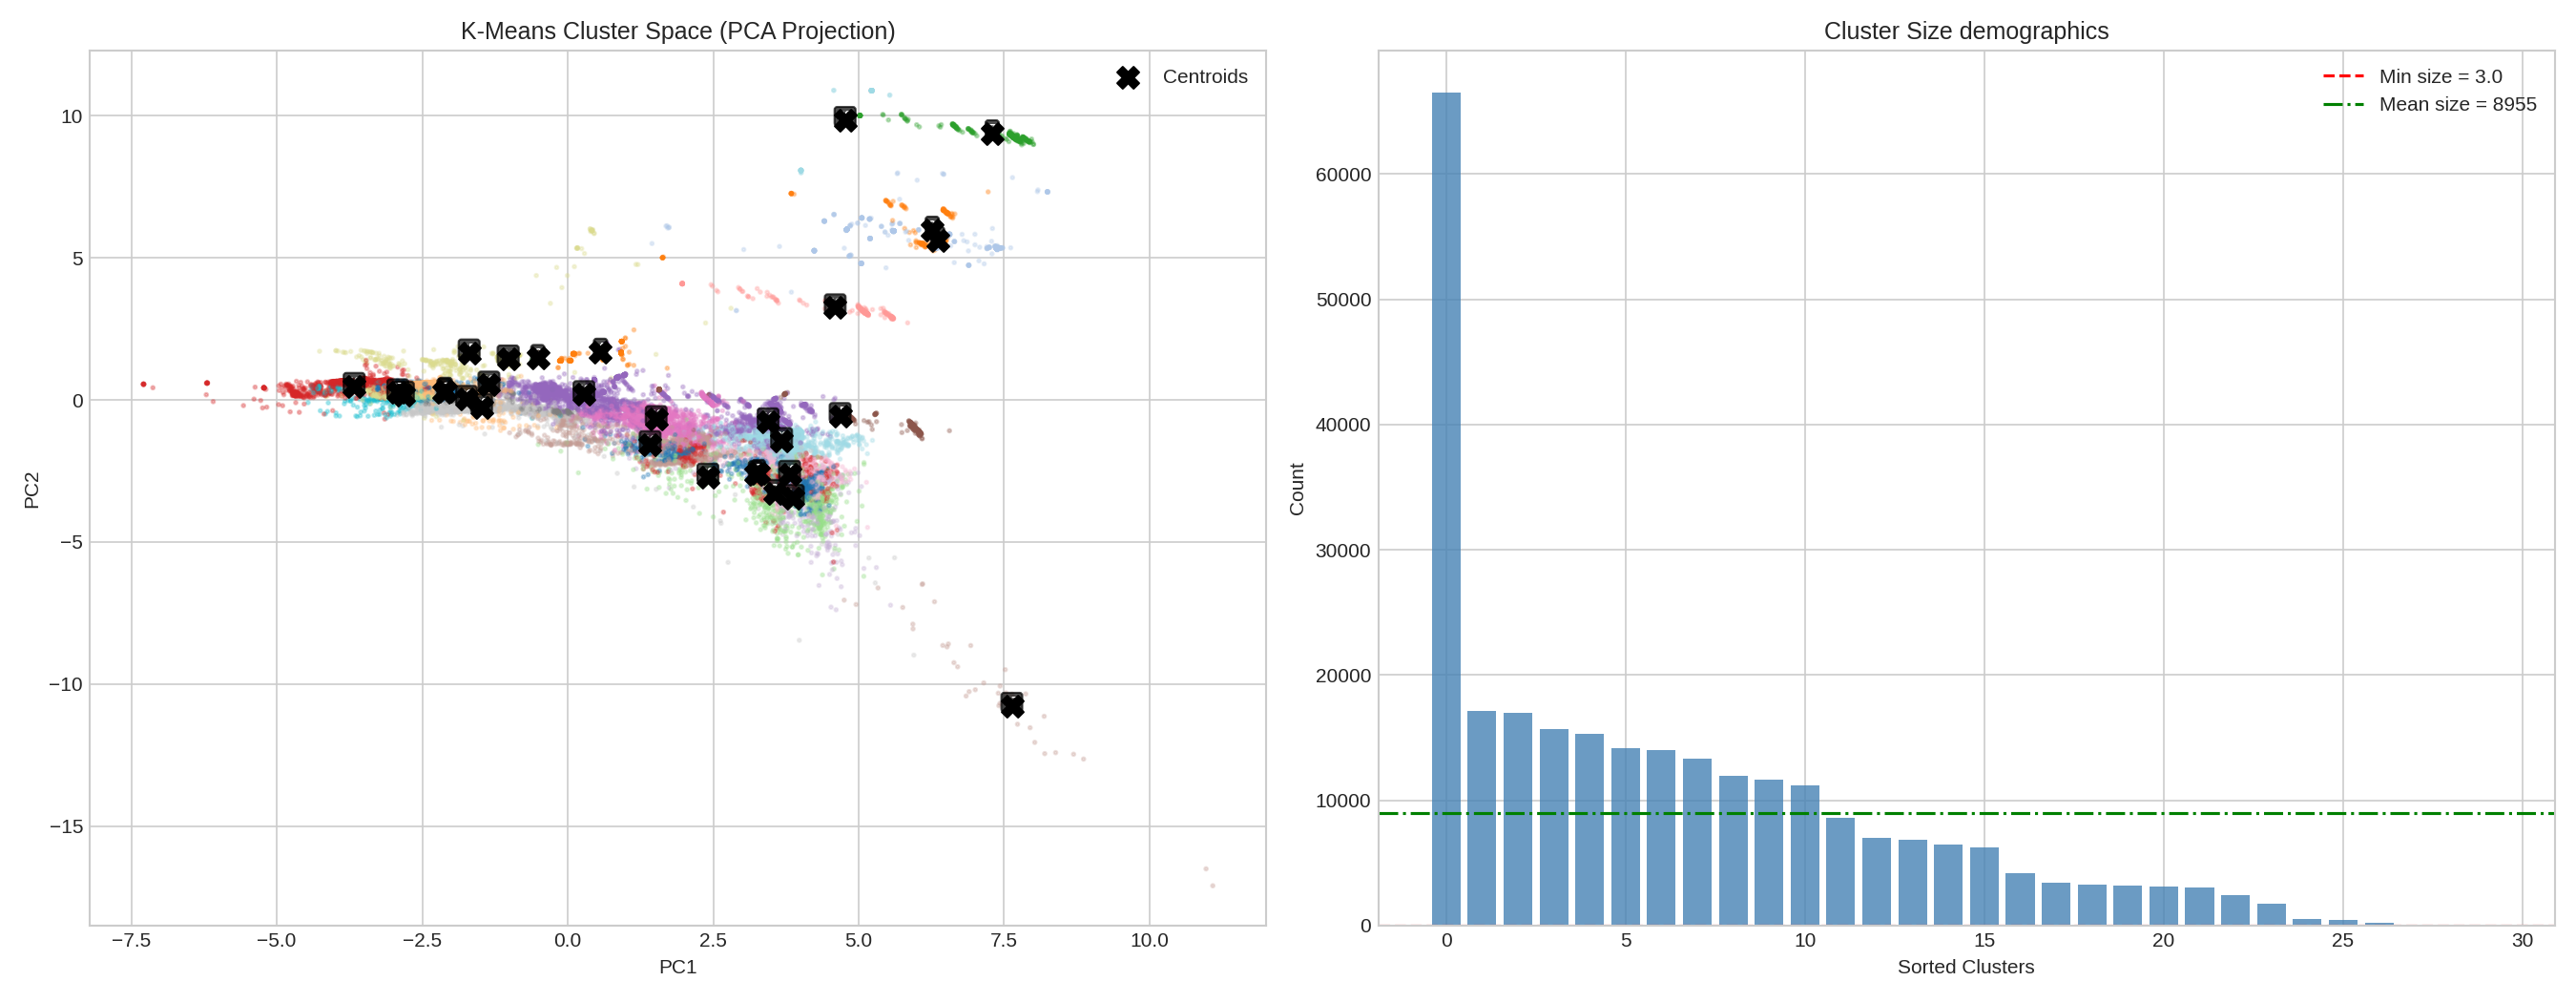
\includegraphics[width=0.48	extwidth]{cluster_visualization.png}
\caption{The K-Means cluster assignments ($K=30$) are shown in PCA space (left) and cluster size distribution (right). The PCA projection shows 30 spatially distinct cluster regions. The size distribution shows one predominant cluster ($66,519$ flows) and a long tail following a power-law distribution typical of web traffic.}
\label{fig:cluster_pca}
\end{figure}

\section{Discussion}\label{sec:discussion}

\paragraph{Why the RF attacker is more difficult to reduce} The RF's reliance on PacketLengthMode (22.63\% importance) is an error that simple proportional dummy injection cannot reliably close. DNS tunneling tools (dns2tcp/DNSCat2) produce flows of extremely uniform packet size---a strong, repeating mode---which is not displaced by the 25\% dummy injection. The CNN, being sensitive to the entire distribution, learns the whole shape by changing its weights, making it more susceptible to partial morphing. A mode-targeted injection strategy---calculating the exact number of dummy queries required to create a new mode---would close this gap and is left for future work.

\paragraph{Dataset scope} The CIRA-CIC-DoHBrw-2020 dataset evaluates binary classification (benign vs. malicious DoH), which is identical to the practical deployment of DNS tunneling detection. For site-level identification (the harder multi-class problem), DoH-Shield can naturally extend the clustering mechanism to $l$-diversity defined over site labels instead of binary classes, and the number of clusters $K$ would be scaled in parallel. Evaluation on a multi-class dataset (Tranco top-100, 40 traces per class) is planned.

\paragraph{Deployability} DoH-Shield requires only basic user-level setup: adding the mitmproxy CA certificate to Firefox and proxying browser traffic to \texttt{localhost:8080}. No root access, browser modifications, or resolver cooperation is needed. It works on commodity hardware (tested on Ubuntu 22.04) and introduces no noticeable browsing latency as dummy queries are fired asynchronously on background threads.

\paragraph{EDNS(0) padding interaction} DoH-Shield's dummy injection is orthogonal to RFC 8467 EDNS(0) payload padding, and the two may be used in conjunction. Combined, they resolve both content-length leakage (via EDNS padding) and statistical flow-level fingerprinting (via DoH-Shield), providing defense-in-depth.

\section{Conclusion}\label{sec:conclusion}
We introduced DoH-Shield, a client-side implementation of DNS-over-HTTPS (DoH) fingerprinting defense using cluster-aware dummy injection, differential privacy timing noise, and adaptive session-key randomization. The system incorporates a new cluster hardening step (Diverse-Neighbor Merging) that eliminates pure clusters and ensures $k$-anonymity ($k_{\min}=343$) over all clusters. We formally prove $P_{\text{attack}} \le 1/k_{\min} + e^{-\varepsilon} = 37.08\%$ (for $\varepsilon=1.0$), which is independent of the sophistication of the attacker. Experimentally, DoH-Shield reduces a Deep Fingerprinting CNN's F1-score from $0.9989$ to $0.1044$ with under 40\% bandwidth overhead, without server cooperation.

Future work includes evaluation against the LASERBEAK Transformer-based WF attacker [15] and open-world evaluation based on Juarez et al. [11] to quantify false positive rates at sites not being monitored.

\paragraph{Availability} The source code, trained models, and the verification suite are available at \url{https://github.com/TARUN-2305/DoH-Sheild}.

\begin{thebibliography}{15}

\bibitem{rfc8484}
P. Hoffman and P. McManus, ``DNS Queries over HTTPS (DoH),'' IETF RFC 8484, Oct. 2018. [Online]. Available: \url{https://www.rfc-editor.org/rfc/rfc8484}

\bibitem{rfc8467}
A. Mayrhofer, ``Padding Policies for Extension Mechanisms for DNS (EDNS(0)),'' IETF RFC 8467, Oct. 2018. [Online]. Available: \url{https://www.rfc-editor.org/rfc/rfc8467}

\bibitem{cira2020}
M. Montazeri Shatoori, L. Davidson, G. Kaur, and A. H. Lashkari, ``Detection of DoH Tunnels using Time-series Classification of Encrypted Traffic,'' in \emph{Proc. 5th IEEE Int. Conf. Cyber Science and Engineering (CyberSci)}, Aug. 2020, pp. 338--345. DOI: 10.1109/CyberSciTech49723.2020.00070

\bibitem{sirinam2018}
P. Sirinam, M. Imani, M. Juarez, and M. Wright, ``Deep Fingerprinting: Undermining Website Fingerprinting Defenses with Deep Learning,'' in \emph{Proc. ACM CCS 2018}, Oct. 2018, pp. 1928--1943. DOI: 10.1145/3243734.3243768

\bibitem{panchenko2022}
A. Panchenko, A. Mitseva, M. Henze, K. Wehrle, and T. Engel, ``Toward practical defense against traffic analysis attacks on encrypted DNS traffic,'' \emph{Computers \& Security}, vol. 119, p. 102734, Aug. 2022. DOI: 10.1016/j.cose.2022.102734

\bibitem{dwork2006}
C. Dwork, F. McSherry, K. Nissim, and A. Smith, ``Calibrating Noise to Sensitivity in Private Data Analysis,'' in \emph{Proc. TCC 2006}, LNCS 3876, pp. 265--284. DOI: 10.1007/11681878\_14

\bibitem{dwork2014}
C. Dwork and A. Roth, ``The Algorithmic Foundations of Differential Privacy,'' \emph{Foundations and Trends in Theoretical Computer Science}, vol. 9, no. 3--4, pp. 211--407, 2014. DOI: 10.1561/0400000042

\bibitem{ldiversity}
A. Machanavajjhala, D. Kifer, J. Gehrke, and M. Venkitasubramaniam, ``l-Diversity: Privacy Beyond k-Anonymity,'' \emph{ACM Trans. Knowledge Discovery from Data}, vol. 1, no. 1, Mar. 2007. DOI: 10.1145/1217299.1217302

\bibitem{sweeney2002}
L. Sweeney, ``k-Anonymity: A Model for Protecting Privacy,'' \emph{Int. J. Uncertainty, Fuzziness and Knowledge-Based Systems}, vol. 10, no. 5, pp. 557--570, 2002. DOI: 10.1142/S0218488502001648

\bibitem{glove}
R. Nithyanand, X. Cai, and R. Johnson, ``Glove: A Bespoke Website Fingerprinting Defense,'' in \emph{Proc. ACM WPES 2014}, pp. 131--134. DOI: 10.1145/2665943.2665960

\bibitem{juarez}
M. Juarez, S. Afroz, G. Acar, C. Diaz, and R. Greenstadt, ``A Critical Evaluation of Website Fingerprinting Attacks,'' in \emph{Proc. ACM CCS 2014}, pp. 263--274. DOI: 10.1145/2660267.2660368

\bibitem{khajavi}
S. Khajavi and J. Wang, ``Lightening the Load: A Cluster-Based Framework for a Lower-Overhead, Provable Website Fingerprinting Defense,'' \emph{arXiv preprint arXiv:2509.01046}, Sep. 2025.

\bibitem{tamaraw}
X. Cai, R. Nithyanand, T. Wang, R. Johnson, and I. Goldberg, ``A Systematic Approach to Developing and Evaluating Website Fingerprinting Defenses,'' in \emph{Proc. ACM CCS 2014}, pp. 227--238. DOI: 10.1145/2660267.2660362

\bibitem{li2024}
Z. Li, S. Zhang, and W. Lou, ``From Fingerprint to Footprint: Exploiting HTTP/2 Key Frame Sequences for Website Fingerprinting on Encrypted DNS Traffic,'' in \emph{Proc. ESORICS 2024}, 2024.

\bibitem{laserbeak}
P. Guo and X. Yuan, ``LASERBEAK: Transformer-based Website Fingerprinting Using Sequential Attention,'' in \emph{Proc. IEEE Security \& Privacy Workshop on Traffic Analysis}, 2024.

\end{thebibliography}
\end{document}
